\documentclass[10pt]{beamer}

\usepackage[T2A]{fontenc}
\usepackage[utf8]{inputenc}
\usepackage[russian,english]{babel}
\usepackage{subfig}
\usepackage[noend]{algorithm,algpseudocode}
\usepackage{amsmath}

\usepackage{booktabs}
\usepackage[scale=2]{ccicons}

\usepackage{pgfplots}
\usepgfplotslibrary{dateplot}

\usepackage{xspace}
\newcommand{\TODO}[1]{\textbf{\textcolor{red}{TODO: #1}}}


\algblockdefx{MRepeat}{EndRepeat}{\textbf{repeat}}{}
\algnotext{EndRepeat}

\algrenewcommand\alglinenumber[1]{\footnotesize #1}
\DeclareMathOperator{\rank}{rank}
\DeclareMathOperator{\sign}{sign}

\newcounter{mycounter}

\newcommand{\myparagraph}{\stepcounter{mycounter}\paragraph{\arabic{mycounter}}}

\title{Лекция 1}
\subtitle{Введение}

\begin{document}

\maketitle

\begin{frame}{Информация по курсу}
  email: machine.teaching@gmail.com \\
  web: \href{http://mit.spbau.ru/sewiki/index.php/Машинное_обучение_2018}{http://mit.spbau.ru/sewiki/index.php/Машинное\_обучение\_2018}\\
\end{frame}

\section{Правила игры}

\begin{frame}{Правила игры}
  \begin{enumerate} [-]  
    \item 13 лекций
    \item 12 опросов по 5 баллов в начале лекции
    \item 8 домашних заданий по 20 баллов при сдаче в первую неделю, 10 баллов при сдаче во вторую неделю
    \item Экзамен 180 баллов
    \bigbreak
    \item Оценки за курс: \alert{320 баллов} -- отлично, \alert{280 баллов} -- хорошо, \alert{240 баллов} -- удовлетворительно
  \end{enumerate}  
\end{frame}

\section{Машинное обучение}

\begin{frame}{Что такое машинное обучение?}
  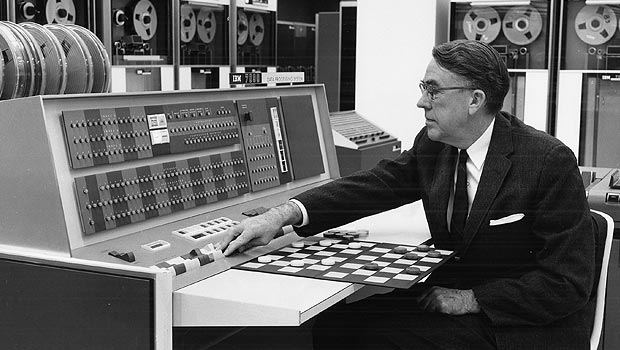
\includegraphics[width=0.5 \linewidth, height=0.5 \textheight, keepaspectratio]{images/samuel}\\
	Arthur Samuel (1959) \\
	\bigbreak
	Field of study that gives computers the ability to learn without being explicitly programmed.
\end{frame}

\begin{frame}{Пример}
  Чем отличается задача \alert{найти кратчайший путь в графе} от\\  \alert{антиспам фильтр}?
\end{frame}

\section{Применение машинного обучения}

{\foot{Recommender system}
\begin{frame}{Рекомендации}
  \centering
  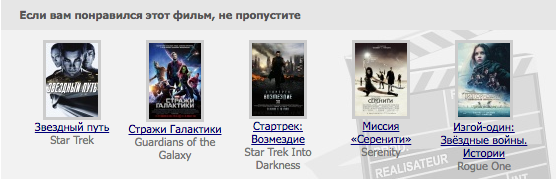
\includegraphics[width=\linewidth, height=\textheight, keepaspectratio]{images/recommendations}\\
\end{frame}
}

{\foot{Information retrieval}
\begin{frame}{Информационный поиск}
  \centering
  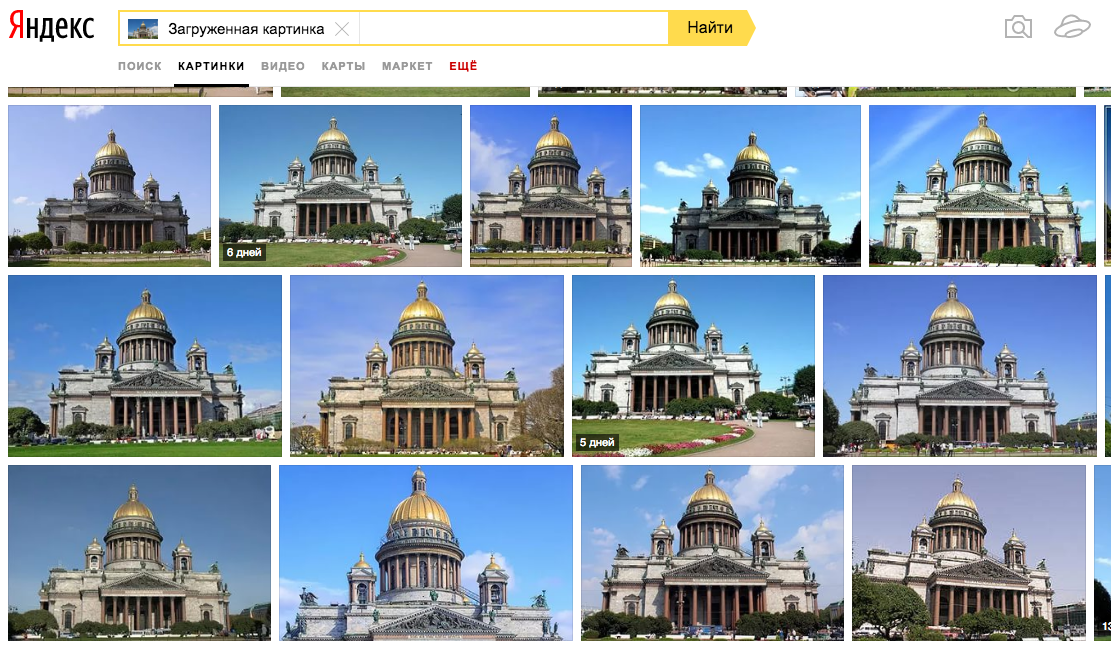
\includegraphics[width=\linewidth, height=\textheight, keepaspectratio]{images/similar_image}\\
\end{frame}
}

{\foot{Image captioning}
\begin{frame}{Подпись изображений}
  \centering
  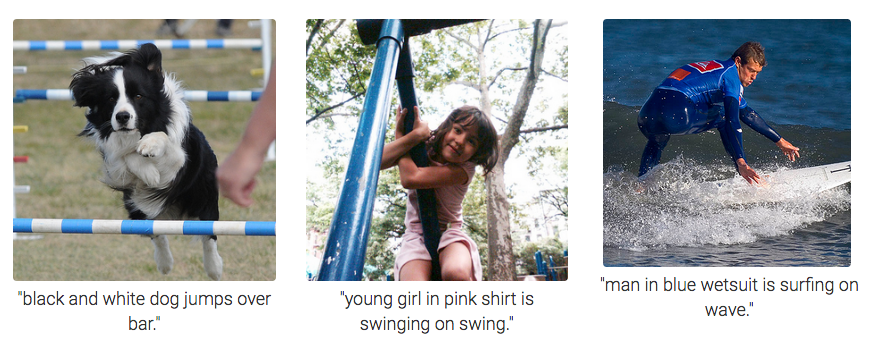
\includegraphics[width=\linewidth, height=\textheight, keepaspectratio]{images/image_captioning}\\
\end{frame}
}

{\foot{Sentiment analysis}
\begin{frame}{Анализ тональности текста}
  \centering
  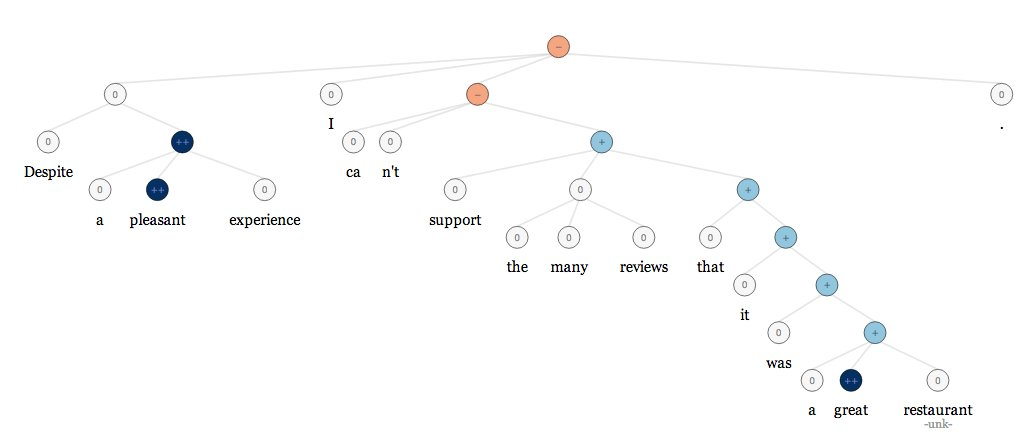
\includegraphics[width=\linewidth, height=\textheight, keepaspectratio]{images/sentiment}\\
\end{frame}
}

{\foot{Instant translation}
\begin{frame}{Машинный перевод}
  \centering
  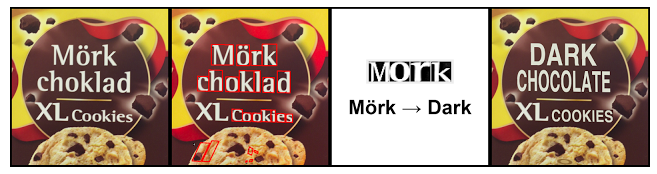
\includegraphics[width=0.9 \linewidth, height=0.9 \textheight, keepaspectratio]{images/translation}\\
\end{frame}
}

{\foot{Self driving car}
\begin{frame}{Беспилотный автомобиль}
  \centering
  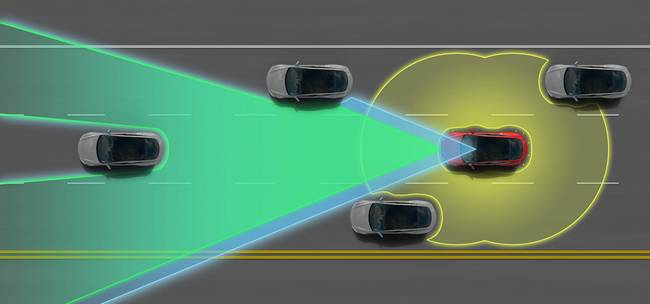
\includegraphics[width=0.9 \linewidth, height=0.9 \textheight, keepaspectratio]{images/self_driving}\\
\end{frame}
}

\section{Какая математика понадобится}

\begin{frame}{Какая математика понадобится?}
	\begin{itemize} [<+->]
	  \item[--] Линейная алгебра
	  \item[--] Теория вероятности
	  \item[--] Математическая статистика 
	  \item[--] Дискретная математика
	  	\item[--] Методы оптимизации 
	\end{itemize}
\end{frame}

\section{Кто уже использовал методы машинного обучения? }

\section{Достаточно ли знать алгоритмы ML и математику?}

\begin{frame}{Что еще надо понимать}
	\begin{itemize} [<+->]
	  \item[--] Когда надо применять ML
	  \item[--] Как сформулировать задачу в терминах ML
	  \item[--] Как выбрать подходящий класс алгоритмов
	  \item[--] Где посмотреть существующие решения
	  \item[--] Как настроить алгоритм
	  \item[--] Как оценить результаты
	\end{itemize}
\end{frame}

\section{Немного истории}

\begin{frame}{История ML}
	\begin{itemize} [<+->]
	  \item[1958] Frank Rosenblatt создает первую искусственную нейронную сеть
	  \item[1959] Arthur Samuel создает первую самообучающуюся шашечную программу для IBM 701
	  \item[1963] Larry Roberts сформулировал тезисы компьютерного зрения
	  \item[1973] James Lighthill. "Искусственный интеллект: Общий обзор"
	  \item[1986] David Rumelhart и Ronald Williams заново открыт и популяризирован алгоритм обратного распространения ошибки
	  \item[1997] Компьютер Deep Blue обыграл чемпиона мира по шахматам Гарри Каспарова
	  \item[2006] Geoffrey Hinton ввел в обиход термин «Deep learning» 
	  \item[2011] Суперкомпьютер IBM Watson одержал победу в телевикторине Jeopardy!
	  \item[2014] Facebook изобрел алгоритм DeepFace для распознавания лиц
	  \item[2016] Программа AlphaGo обыграла чемпиона мира по игре в го Lee Se-dol в четырех партиях из пяти
	\end{itemize}
\end{frame}

{\foot{Moravec's paradox}
\begin{frame}{Зима AI}
	\begin{itemize} [<+->]
	  \item[--] Проблема комбинаторного взрыва
	  \item[--] Низкая производительность компьютеров
	  \item[--] Проблема представлений знаний “здравого смысла”
	  \item[--] Парадокс Моравека
	\end{itemize}
\end{frame}
}

\section{Типы машинного обучения}

\begin{frame}{Типы машинного обучения}
	\begin{enumerate}
	  \item С учителем
	  \item Без учителя
	  \item С частичным привлечением учителя
	  \item Обучение с подкреплением
	  \item Активное обучение
	\end{enumerate}
\end{frame}

{\foot{Supervised learning}
\begin{frame}{Обучение с учителем}
  	$X$ - множество объектов \\
	$Y$ - множество ответов \\
	Обучающая выборка: ${X^l = (x_i, y_i)_{i=1}^l}$ \\  
	\bigbreak
	\bigbreak
	\alert{Задача}: Построить алгоритм ${a \colon X \rightarrow Y}$
\end{frame}
}

{\foot{Supervised learning. Classification}
\begin{frame}{Обучение с учителем. Классификация }
	$X$ - множество объектов \\
	$Y$ - множество классов \\
	Обучающая выборка: ${X^l = (x_i, y_i)_{i=1}^l}$ \\ 
	\bigbreak
	\bigbreak
	\alert{Задача}: Построить алгоритм ${a \colon X \rightarrow Y}$, способный классифицировать произвольный объект ${x \in X}$.
\end{frame}
}

{\foot{Supervised learning. Classification}
\begin{frame}{Обучение с учителем. Классификация}
  \centering
  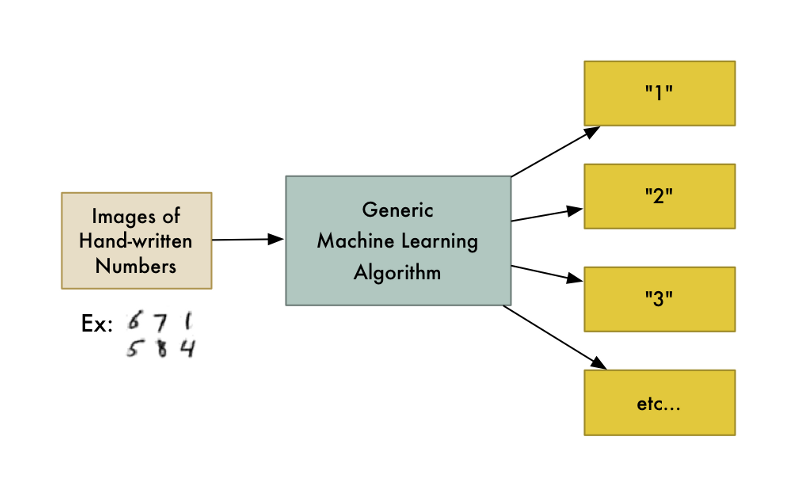
\includegraphics[width=0.9 \linewidth, height=0.9 \textheight, keepaspectratio]{images/mnist}\\
\end{frame}
}

{\foot{Supervized learning. Regression}
\begin{frame}{Обучение с учителем. Регрессия}
  $X$ - множество объектов \\
	$Y$ - множество ответов ${(Y \in \mathbb{R})}$\\
	Обучающая выборка: ${X^l = (x_i, y_i)_{i=1}^l}$ \\ 
	Существует неизвестная целевая зависимость $y^*: X \rightarrow Y$
	\bigbreak
	\bigbreak
	\alert{Задача}: Построить алгоритм ${a \colon X \rightarrow Y}$, аппроксимирующий целевую зависимость $y^*$
\end{frame}
}

{\foot{Supervized learning. Regression}
\begin{frame}{Обучение с учителем. Регрессия}
  \centering
  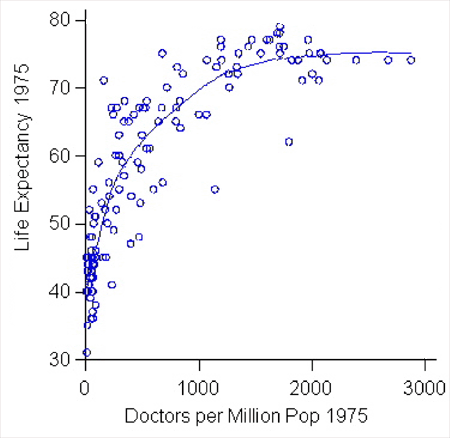
\includegraphics[width=0.7 \linewidth, height=0.7 \textheight, keepaspectratio]{images/regression}\\
\end{frame}
}

\section{Обучение без учителя}

{\foot{Unsupervised learning}
\begin{frame}{Обучение без учителя}
  \centering
  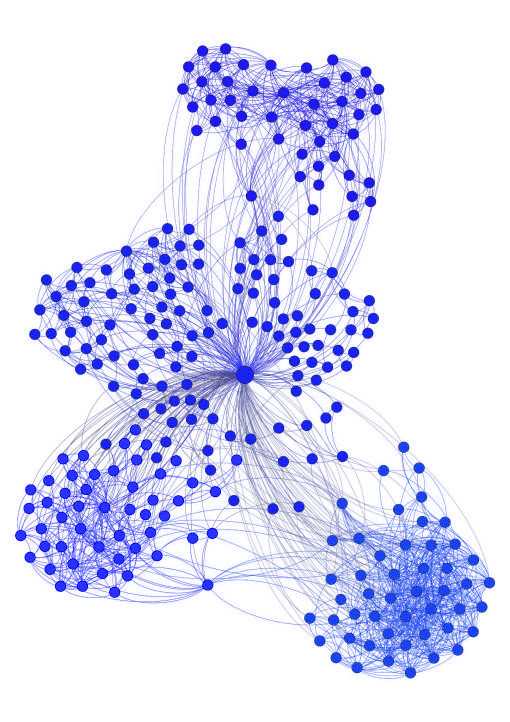
\includegraphics[width=0.9 \linewidth, height=0.9 \textheight, keepaspectratio]{images/clustering1}\\
\end{frame}
}

{\foot{Unsupervised learning}
\begin{frame}{Обучение без учителя}
  \centering
  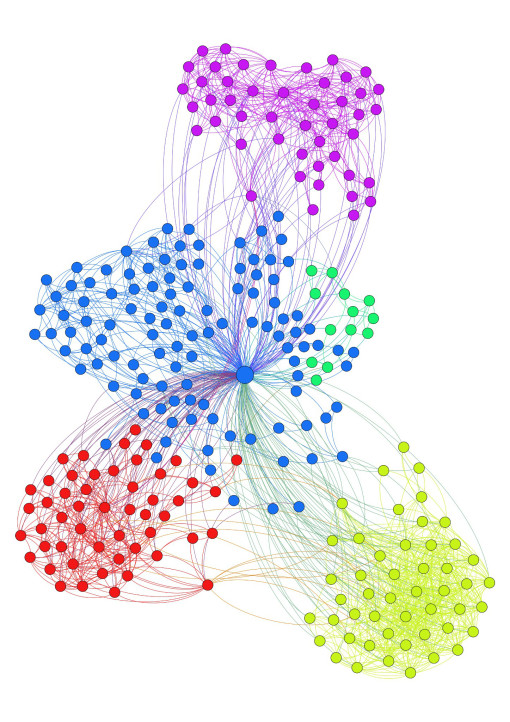
\includegraphics[width=0.9 \linewidth, height=0.9 \textheight, keepaspectratio]{images/clustering}\\
\end{frame}
}


{\foot{Unsupervised learning}
\begin{frame}{Обучение без учителя}
  $X$ - множество объектов \\
	Обучающая выборка: ${X^l = \left\{x_i\right\}_{i=1}^l}$ \\ 
	\bigbreak
	\bigbreak
	\alert{Задача}: Обнаружить внутренние взаимосвязи, зависимости, закономерности, существующие между объектами.
\end{frame}
}

\section{Обучение с частичным привлечением учителя}

{\foot{Semi-supervised learning}
\begin{frame}{С частичным привлечением учителя}
  $X$ - множество объектов \\
	$Y$ - множество ответов \\
	Обучающая выборка: ${X^l = (x_i, y_i)_{i=1}^l}$, ${X^u = \left\{x_i\right\}_{i=1}^u}$ \\  
	\bigbreak
	\bigbreak
	\alert{Задача}: Построить алгоритм ${a \colon X \rightarrow Y}$
\end{frame}
}

{\foot{Semi-supervised learning}
\begin{frame}{С частичным привлечением учителя}
  \centering
  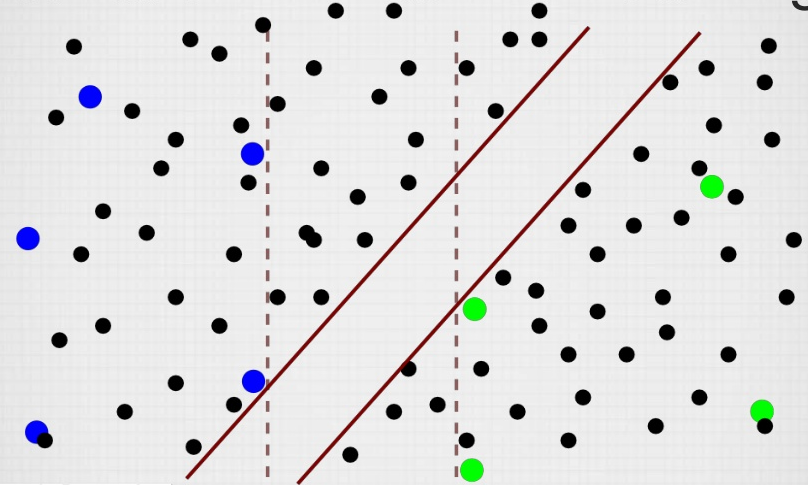
\includegraphics[width=0.9 \linewidth, height=0.9 \textheight, keepaspectratio]{images/semi}\\
\end{frame}
}

\section{Активное обучение}

{\foot{Active learning}
\begin{frame}{Активное обучение}
  $X$ - множество объектов \\
	$Y$ - множество классов \\
	Обучающая выборка: ${X^l = (x_i, y_i)_{i=1}^l}$ \\ 
	Получение дополнительных ответов $y_i$ \alert{дорого}.
	\bigbreak
	\bigbreak
	\alert{Задача}: Построить алгоритм ${a \colon X \rightarrow Y}$, использовав как можно меньше дополнительных элементов.
\end{frame}
}

{\foot{Active learning}
\begin{frame}{Активное обучение}
  \centering
  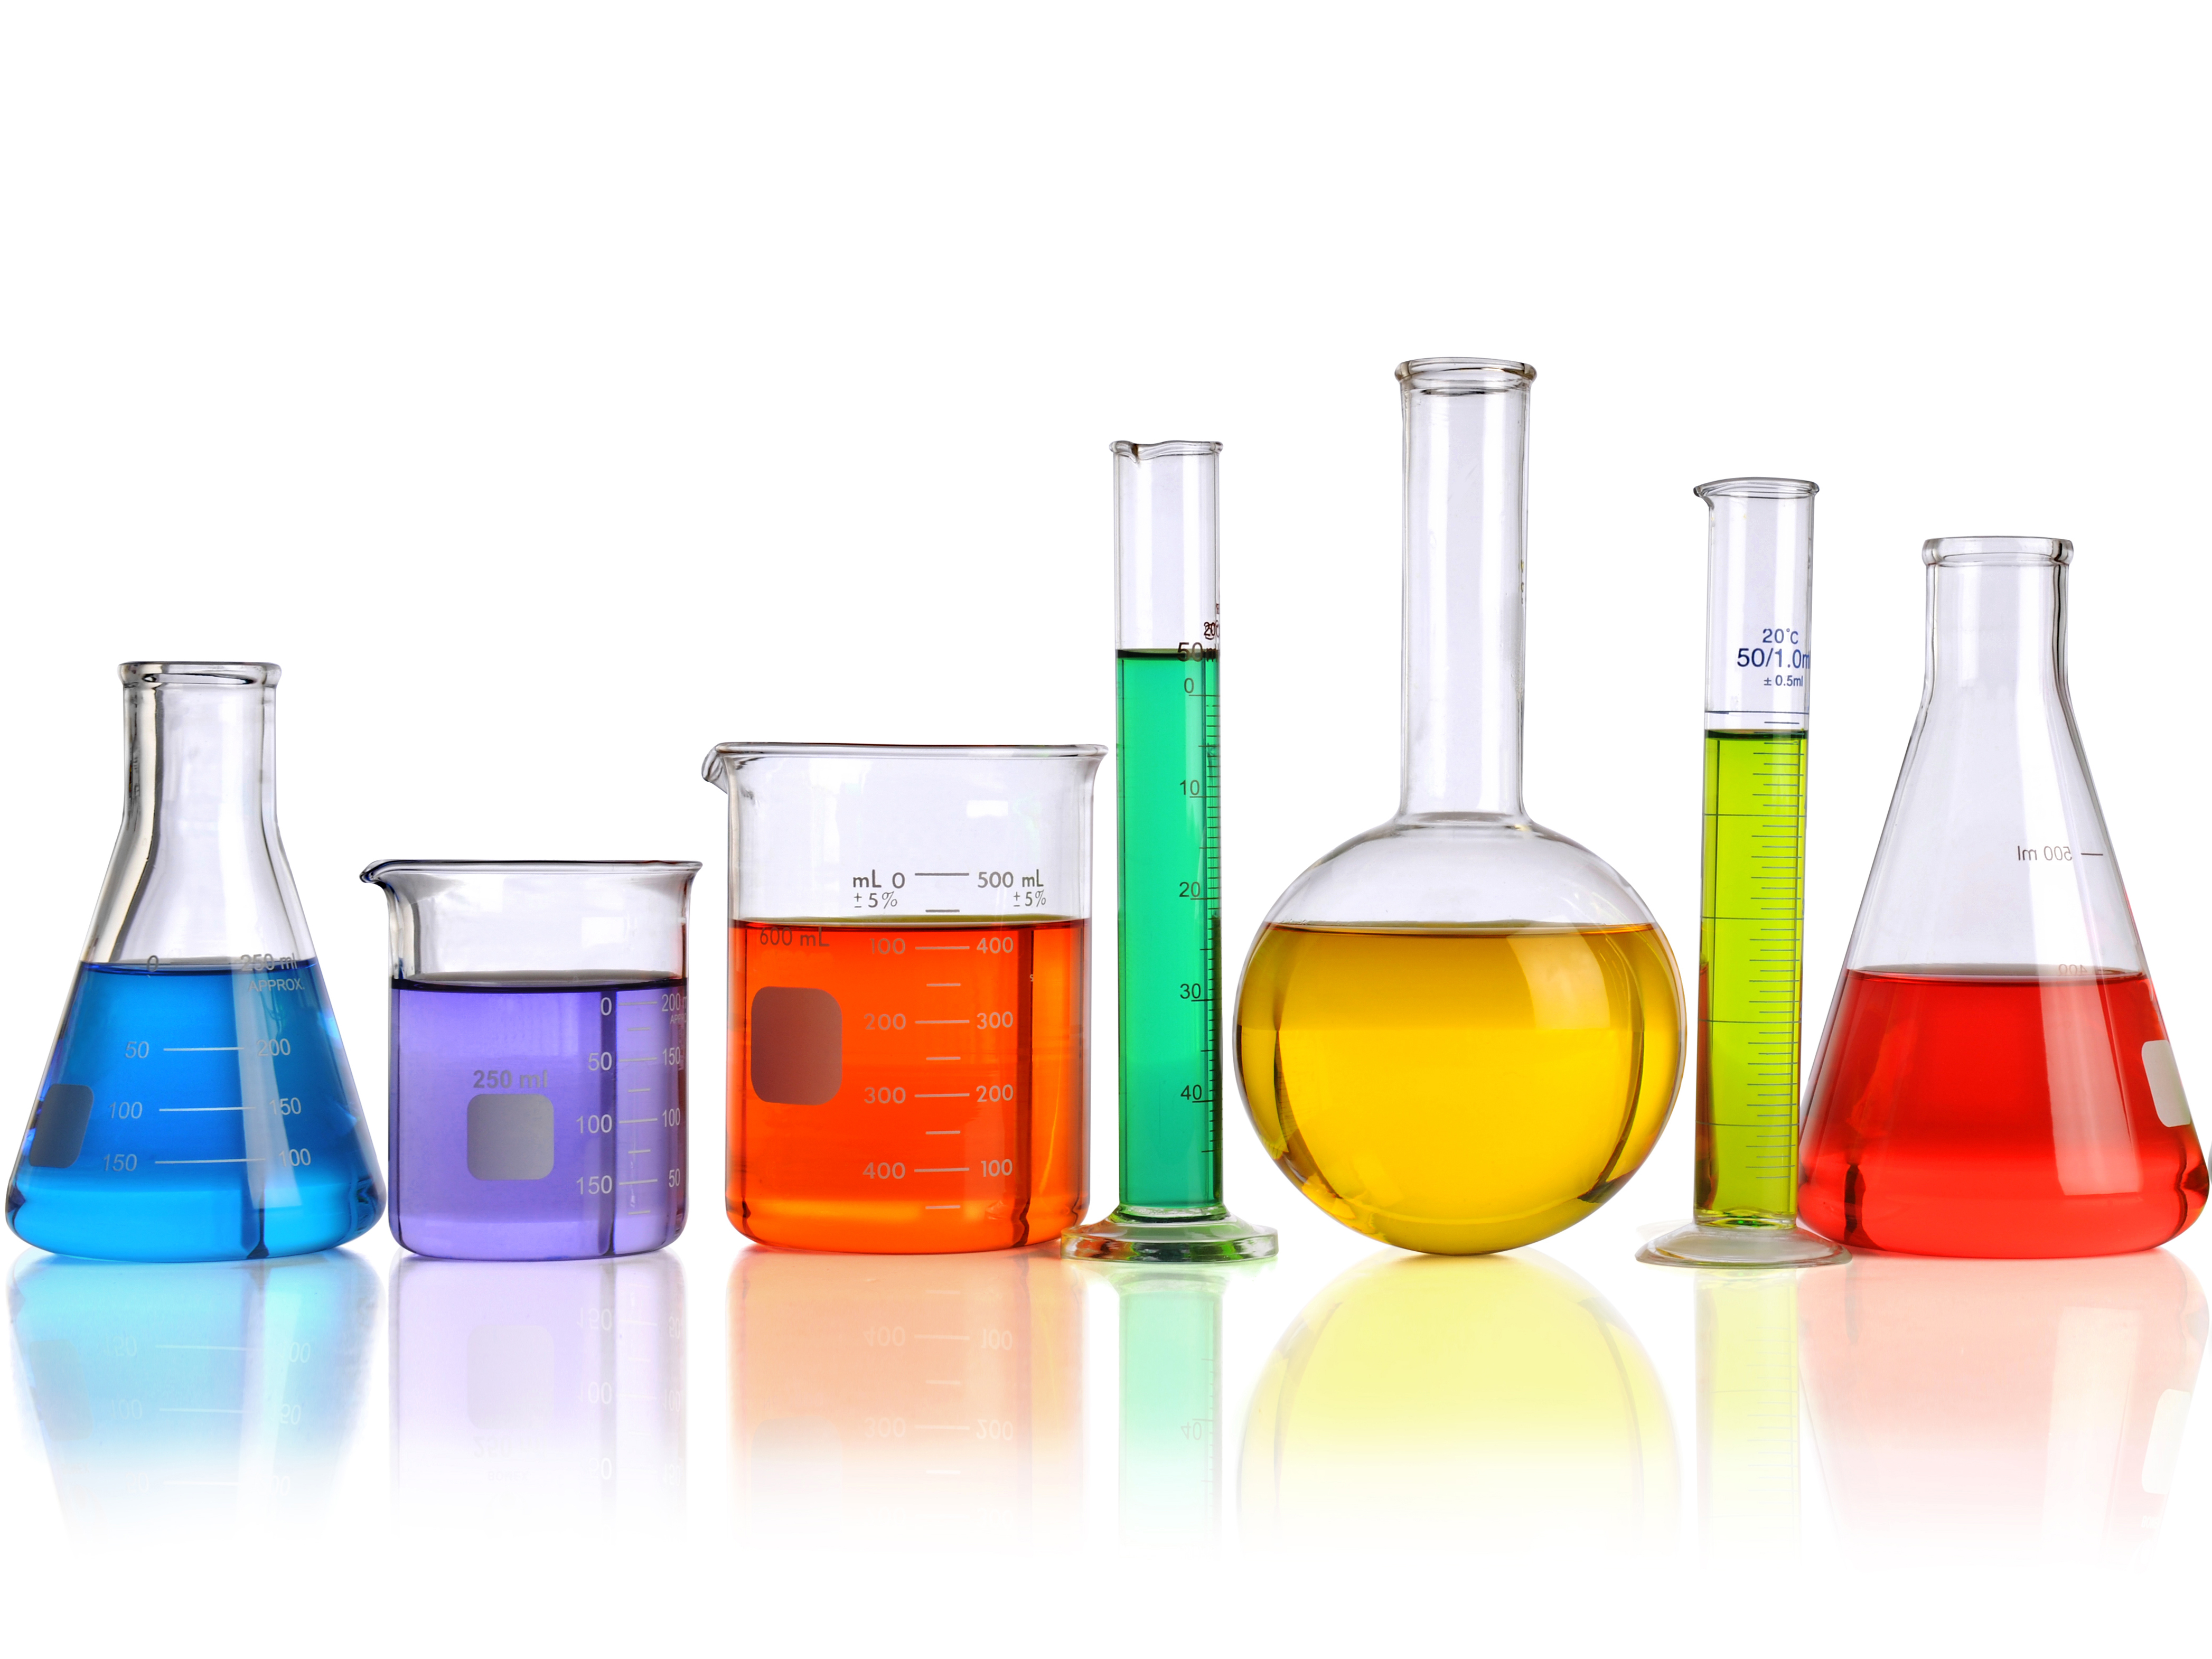
\includegraphics[width=0.9 \linewidth, height=0.9 \textheight, keepaspectratio]{images/active}\\
\end{frame}
}

\section{Обучение с подкреплением}

{\foot{Reinforcement learning}
\begin{frame} {Обучение с подкреплением}
  $S$ -- множество состояний окружения\\
  $A$ -- множество действий агента\\
  $R$ -- множество "выигрышей"
  \bigbreak
	\bigbreak
	\alert{Задача}: Построить алгоритм ${a \colon S \rightarrow A}$, который максимизирует общий "выигрыш"
\end{frame}
}

{\foot{Reinforcement learning}
\begin{frame} {Обучение с подкреплением}
  \centering
  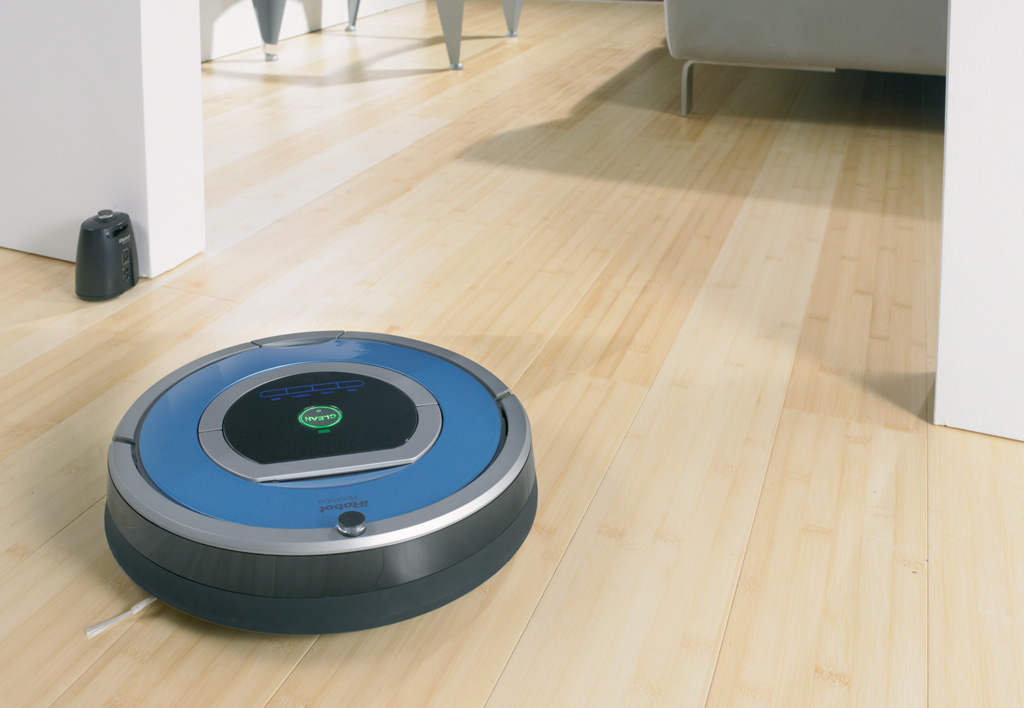
\includegraphics[width=0.9 \linewidth, height=0.9 \textheight, keepaspectratio]{images/roomba}\\
\end{frame}
}

\section{Типы признаков}

\begin{frame}{Типы признаков}
	${f: X \rightarrow D_f}$
	\begin{itemize} [<+->]
	  \item[--] Бинарные (${D_f = \left\{ 0, 1 \right\} }$)
	  \item[--] Номинальные (${D_f}$ -- конечное множество)
	  \item[--] Порядковые (${D_f}$ -- конечное упорядоченное множество)
	  \item[--] Количественные (${D_f = \mathbb{R} }$)
	\end{itemize}
\end{frame}

\begin{frame}{Типы признаков (примеры)}
	\begin{itemize} [<+->]
	  \item[--] Бинарные (Пол, наличие боли в спине, в сознании ли пациент)
	  \item[--] Номинальные (Тип боли: колющая, режущая, ноющая)
	  \item[--] Порядковые (Общее состояние больного: удовлетворительное, средней тяжести, тяжелое, крайне тяжелое)
	  \item[--] Количественные (Температура тела, пульс, артериальное давление)
	\end{itemize}
\end{frame}

\begin{frame}{Применение ML}
	\begin{itemize} [<+->]
	  \item[--] Академическое
	  \item[--] Практическое
	\end{itemize}
\end{frame}

\begin{frame}{Что читать/смотреть}
  \href{http://www.machinelearning.ru/wiki/images/6/6d/Voron-ML-1.pdf}{Курс К. В. Воронцова}\\
	\href{https://yandexdataschool.ru/edu-process/courses/machine-learning}{Видеолекции ШАД}\\
	Christopher M. Bishop "Pattern Recognition and Machine Learning"\\
	G. James, D. Witten, T. Hastie, R. Tibshirani: "An Introduction to Statistical Learning" 	\\
	\href{http://work.caltech.edu/telecourse.html}{Professor Yaser Abu-Mostafa MOOC}
\end{frame}

\begin{frame}[standout]
  Вопросы?
\end{frame}

\appendix

\begin{frame}{На следующей лекции}
	\begin{itemize}
	  \item[--] Метод ближайших соседей
	  \item[--] Гипотеза компактности
	  \item[--] Обобщенный метрический классификатор
	  \item[--] Проклятие размерности  
	  \item[--] Отбор эталонов     
	\end{itemize}
\end{frame}

\end{document}